\section{The MBSecMon Framework}\label{sec:mbsecmonFramework}
The Model-based Security/Safety Monitor (MBSecMon) Framework~\cite{Patzina2011} has been developed as a generic approach to build tool chains for monitor generation.
In this section, we show how this framework has been tailored to fit seamlessly in a model-based AUTOSAR development process and solve the challenges that are raised in Sect.~\ref{sec:introduction}.
This overcomes the current lack of model-based monitoring support in AUTOSAR tool chains that we attested in Sect.~\ref{sec:relatedWork}.
%To cope with the high degree of abstraction between the model and the implementation an instrumentation tool~\cite{Piper2012} for AUTOSAR specifications is used.

\subsection{Example: Automatic Transmission Controller}\label{sec:example}
The example used throughout this paper focuses on monitoring the communication between AUTOSAR software components (SW-Cs). %, despite the MBSecMon framework is not limited to this application scenario.
The AUTOSAR system is modeled with the tool OptXware Embedded Architect\footnote{OptXware: http://www.optxware.com} and the implementation of the subsystems is generated by the AUTOSAR code generation of MathWork's Embedded Coder plugin for Simulink.
 
The implementation of the example system is based on the \emph{Automatic Transition Controller} demo project~\cite{TheMathWorks2012}, shipped with Matlab/Simulink.
As depicted in the system model in Fig.~\ref{fig:simulinkExample}, this model describes the internal behavior of three application-level software components, \emph{ShiftLogic}, \emph{Transmission}, and \emph{Engine}, based on the input values \emph{Throttle} and \emph{BrakeTorque} and the interaction between these components.
Influences such as aerodynamics and drag friction of the wheels are represented by the \emph{Vehicle} block.    
%As source for an realistic but not too complicated example model, depicted in Fig.~\ref{fig:simulinkExample}, the Automatic Transmission Demo project of Matlab/Simulink is used.
To comply with the needs of the AUTOSAR code generation provided by Embedded Coder, the behavioral model has been adapted by replacing all continuous with discrete blocks.
The generated code serves as the behavioral implementation of the skeleton generated by the AUTOSAR tool OptXware Embedded Architect.    
\begin{figure}[tb]
\begin{center}
  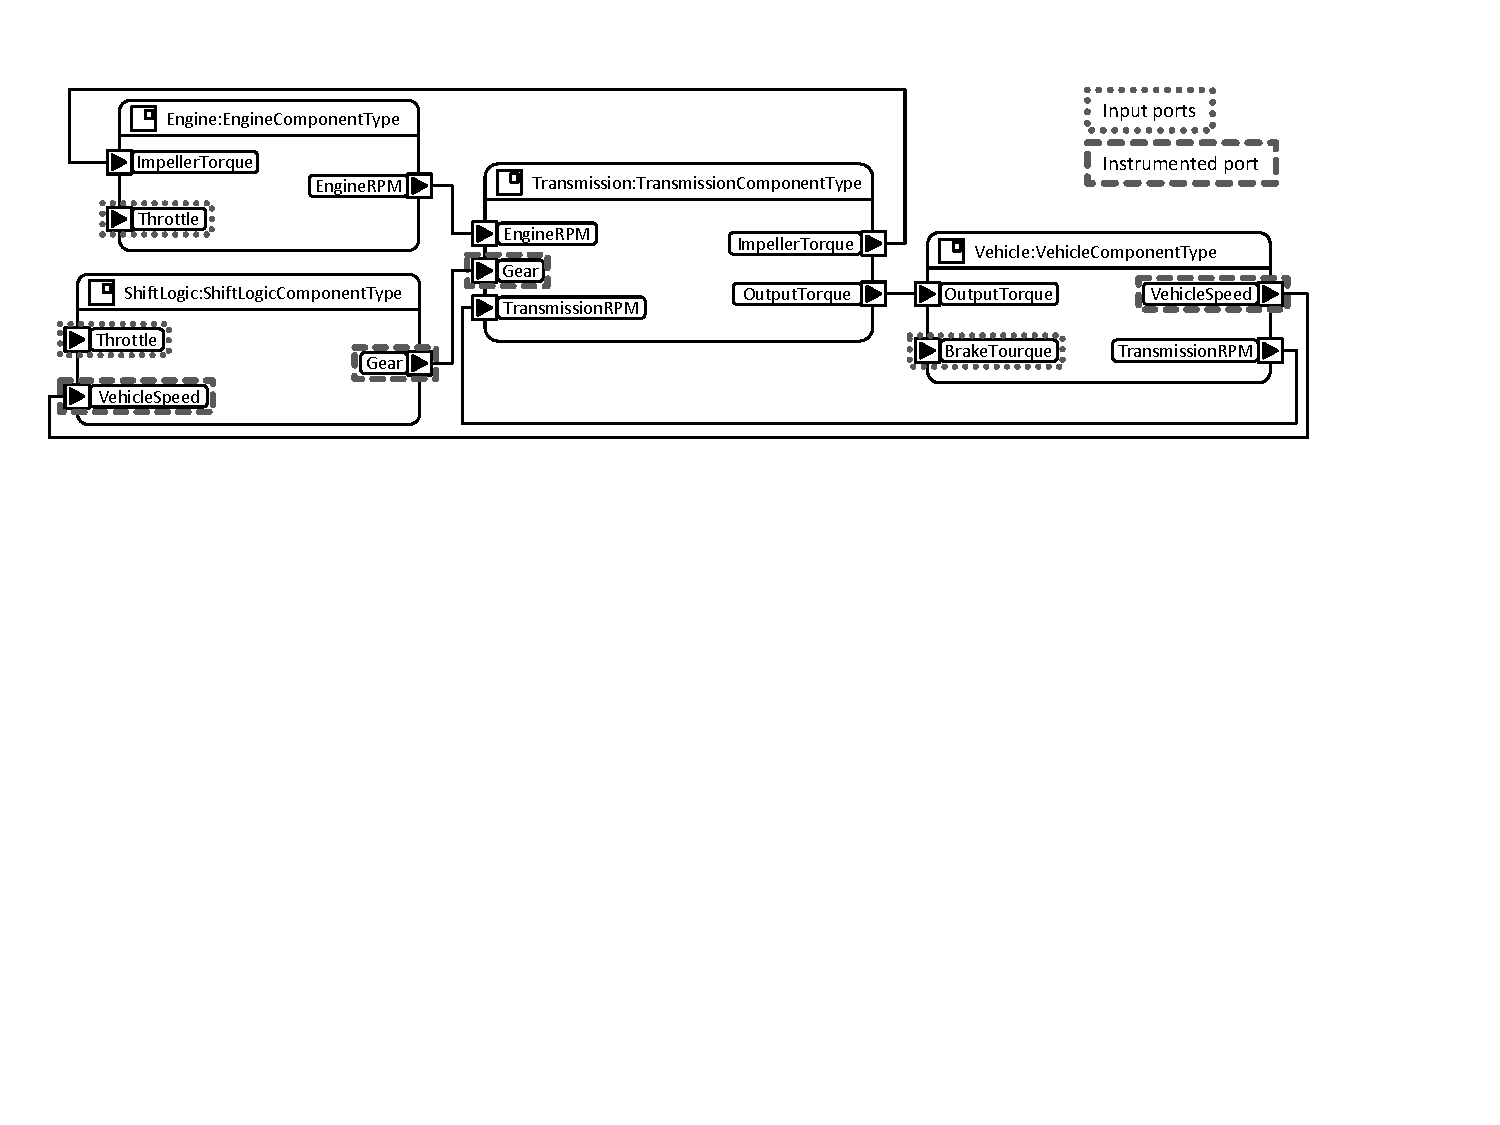
\includegraphics[width=1\textwidth]{AutomaticTransmission.pdf}
  \caption{AUTOSAR example model of an automatic transmission}
  \label{fig:simulinkExample}
\end{center}
\end{figure}
For the asynchronous communication between the components, the sender-receiver communication pattern is used.
%, where the sender does not know the identity and the number of the receivers.
%This pattern is intended to support the transferability of software components.
%auskommentiert, da die transferability/code reuse durch den VFB gew�hrleistet wird, nicht so sehr durch sender/receiver pattern
%The system consists of three components and one component that simulates the behavior of the vehicle.
%As external inputs the throttle and the brake torque are fed into the system and the outputs are throttle, engine RPM and the vehicle speed.
 
%Modeling of component structure and communication channels in OptXware Embedded Architect
%system and implementation from MATLAB model by separation of components and integration into AUTOSAR simulation code 
%- scheduling?

\subsection{The Tailored Monitor Generation Process for AUTOSAR}
%Explanation of the tailored MBSecMon Process in Fig.~\ref{fig:mbsecmonProcess}.
%\usepackage{graphics} is needed for \includegraphics
\begin{figure}[tb]
\begin{center}
  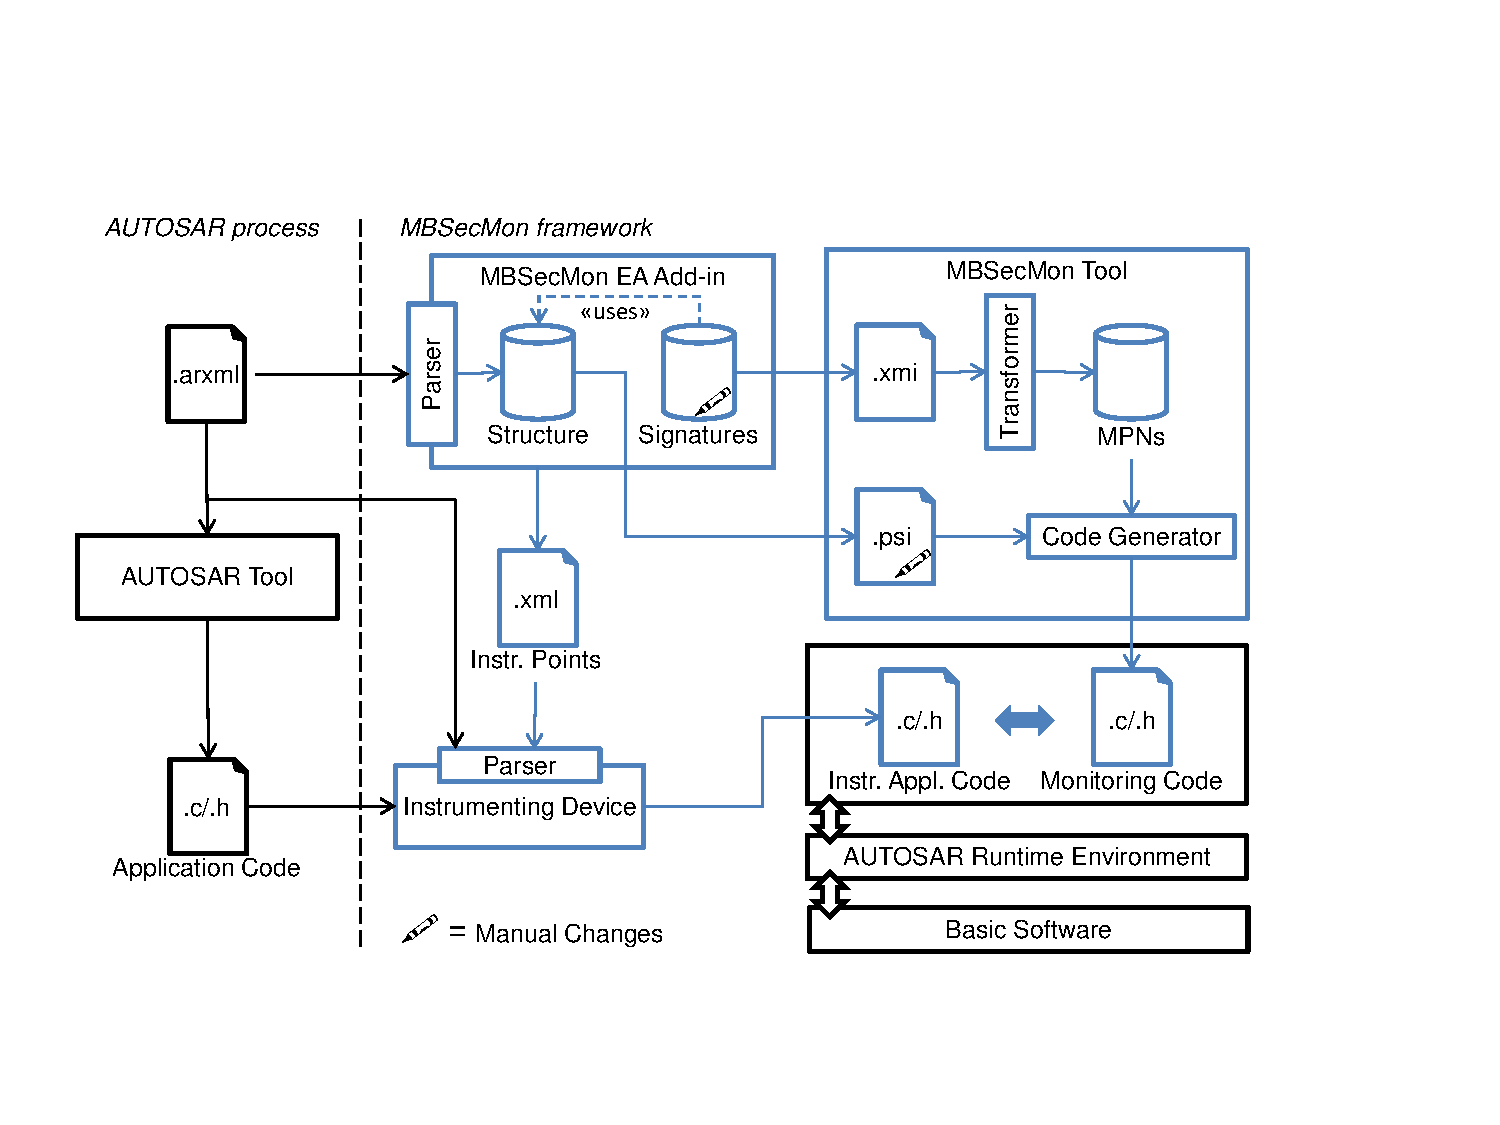
\includegraphics[width=0.75\textwidth]{MBSecMonProcess}
  \caption{MBSecMon framework embedded in AUTOSAR development process}
  \label{fig:mbsecmonProcess}
\end{center}
\end{figure}
The generic MBSecMon development tool chain has been extended to enable a seamless integration into the AUTOSAR development process.    
Figure~\ref{fig:mbsecmonProcess} depicts on the left side the original simplified AUTOSAR development process, starting with the system structure description persisted in the AUTOSAR XML format (ARXML).
This file is used by the AUTOSAR tool chain to generate the RTE and a code skeleton for the implementation of the SW-Cs, which  is supplied by the Simulink code generator. The final code is usable in an AUTOSAR simulation environment or directly on the Electronic Control Unit (ECU) of a vehicle.

On the right-hand side of Fig.~\ref{fig:mbsecmonProcess}, the framework is depicted that embeds the monitor generation tool chain in the AUTOSAR development process.
%As source documents an ARXML file that describes the component view of the system exists.
%At first, we will give an overview of the process for generating monitors.
The specification of monitor signatures is achieved with the help of a tailored version of the UML2 modeling tool Enterprise Architect\footnote{SparxSystems Enterprise Architect: http://www.sparxsystems.com} (EA).
This tool has been extended by an add-in that allows the modeling of eLSCs (\emph{Signatures}) depending on the imported component diagram view (\emph{Structure}) of the AUTOSAR system.% that has been persisted as an ARXML file.
%The structure of the AUTOSAR system is imported from the ARXML file into Enterprise Architect.
%Based on the imported component view of the model \emph{signatures} described by eLSCs are modeled.
The modeled signatures are then exported together with additional platform specific information (PSI) extracted from the imported AUTOSAR model.
Additionally, the \emph{MBSecMon add-in} analyses the modeled signatures for needed \emph{instrumentation points} in the AUTOSAR application code and persists this information in an XML file. 
Through a graph-based model-to-model transformation~\cite{Patzina2012}, the exported representations of the signatures are transformed in the formally defined Monitor Petri nets (MPNs)~\cite{Patzina2010} that serve as an intermediate language used for a straight-forward code generation.
The code generator translates the signatures, represented as MPNs, incorporating the additional information (PSI), to monitoring code.
This monitor is stimulated by calls of its interfaces. 
Therefore, the \emph{instrumenting device} uses the AUTOSAR system specification, together with the \emph{instrumentation points} file, to instrument the application code.
The instrumentation is realized via interface wrappers, which intercept the communication between two components.
A detailed description of the instrumentation of the interfaces of AUTOSAR components with wrappers is given in~\cite{Piper2012}.

This process allows for specifying and automatically generating monitors on an abstract level based on the system information provided by the AUTOSAR development process. 
Only the specification for the monitors has to be modeled using the MBSecMon add-in and the platform specific information has to be extended by the system engineer.   
In the following, based on the example in Sect.~\ref{sec:example}, this process and the necessary adaptation based on the identified challenges are described in detail. 
% Extensions for AUTOSAR
% \begin{itemize}
%   \item import for component diagrams from ARXML
%   \item restriction of modeling freedom, based in imported information
%   \item extension of exported PSI-File for code generation
%   \item export information for instrumentation 
%   \item code generation
%   \begin{itemize}
%     \item type safe AUTOSAR conform interfaces
%     \item translation of external AUTOSAR events to internal monitor events
%  \end{itemize}
% \end{itemize}

\subsubsection{Challenge \ref{itm:integrationExisting}: Integrating existing development fragments.}%$~~$\\
In the AUTOSAR development process, the system structure is modeled at a high abstraction level, describing the  software components (SW-C), their ports with specified data types, and the connections between the ports. 
The generated monitors should observe the communication between these SW-Cs.
Therefore, a component view of the AUTOSAR system should be used to support the modeling of signatures.   

\textit{MBSecMon process:} 
The MBSecMon EA add-in incorporates an ARXML parser that imports the AUTOSAR software component structure, which has been modeled in an AUTOSAR system-level editing tool, such as OptXware Embedded Architect.
Derived from this data, the add-in creates an UML component diagram as shown in Fig.~\ref{fig:autosarsystem} that includes the components, the ports and a connector representation based on the AUTOSAR naming scheme.
Additional system information such as the names of the connectors and ports are stored as tagged values in the model elements and are abbreviated in the diagram view for a clear presentation.
\begin{figure}[tb]
\begin{center}
  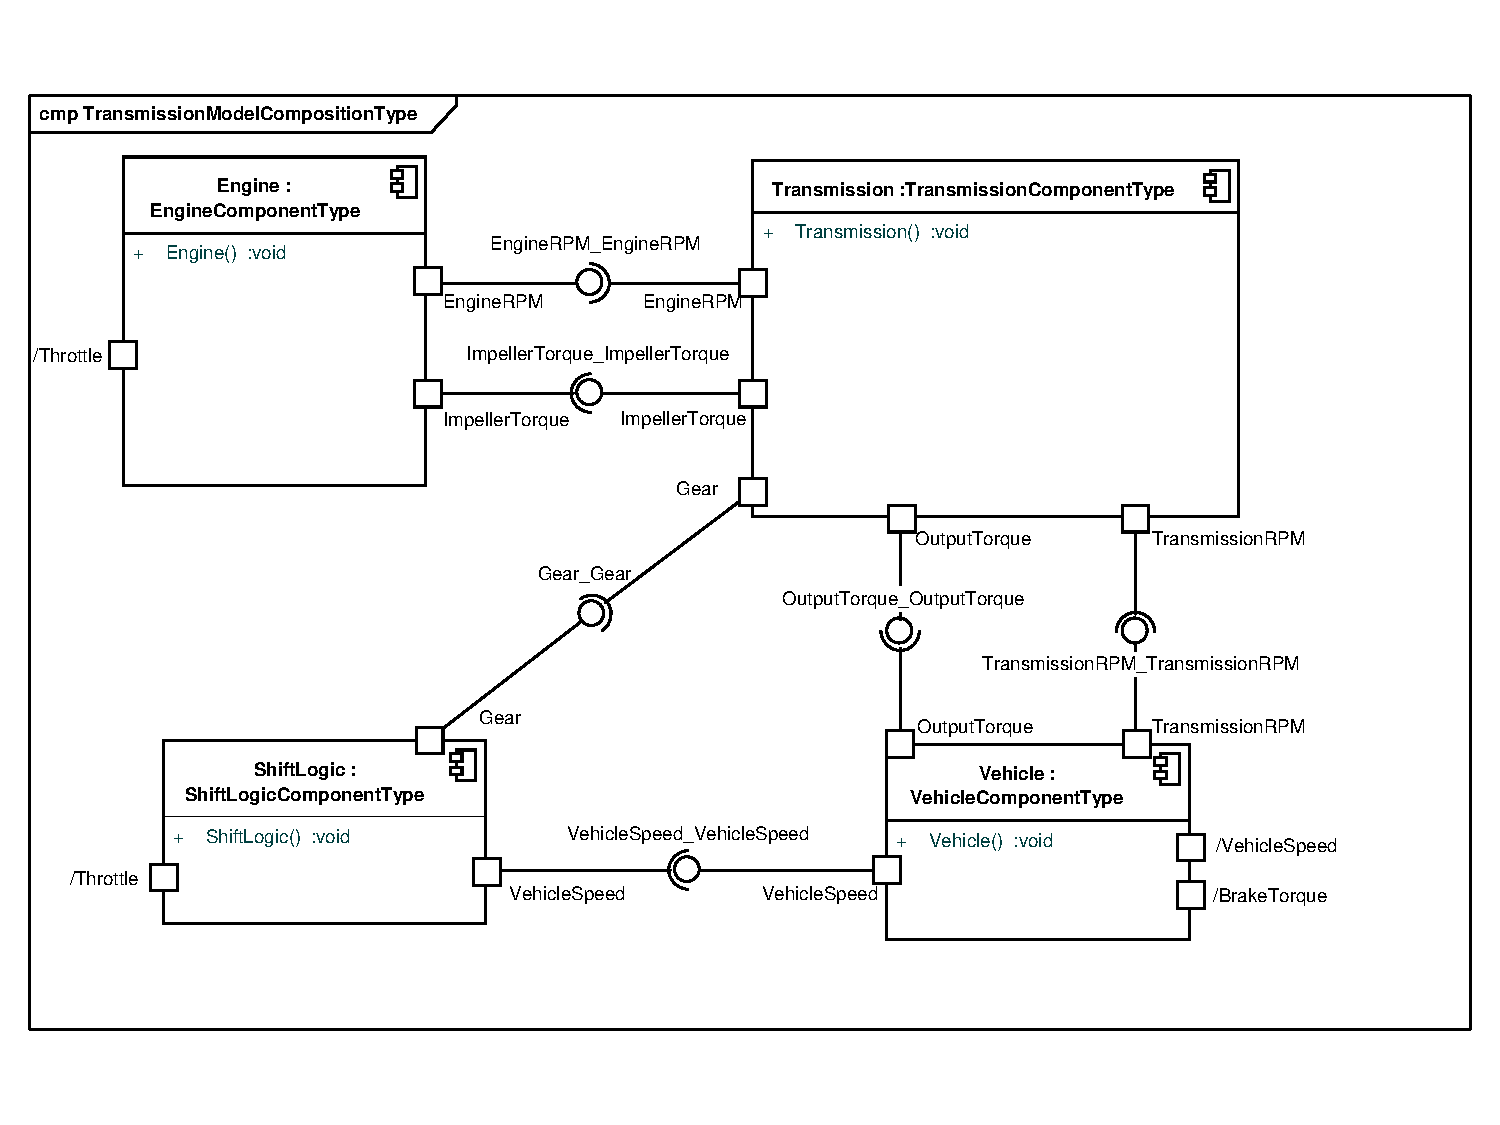
\includegraphics[width=.9\textwidth]{AUTOSARSystem_Componentdiagram}
  \caption{UML component diagram of the system imported to EA}
  \label{fig:autosarsystem}
\end{center}
\end{figure}

\textit{Example:}
The software components in Fig.~\ref{fig:autosarsystem} comply to the blocks of the Simulink model used to generate the implementation of the application code.
This model is used in the MBSecMon development process to describe the allowed and forbidden communication sequences between the components as signatures.   
 
 
\subsubsection{Challenge \ref{itm:datatypesafety}: Providing type safety.}%$~~$\\
In the AUTOSAR development process and in the  automotive domain, specialized data types are used. % to secure data integrity.
This allows for limiting the value range of these data types and prevents wrong assignments such as storing a speed value in a variable intended for the impeller torque.
Generated monitors have to obey this implicit safety mechanism that is inherent in the AUTOSAR standard. 

\textit{MBSecMon process:} 
The special data types provided by the AUTOSAR system specification are imported along with the component diagrams and stored in its ports.  
While modeling the signatures, the developer's choice is constrained to these data types.
These are further used in the monitor generation process and result in type safe monitoring code.

 
\textit{Example:} 
In the ARXML file the data type for the vehicle speed, shown in Listing~\ref{lst:arxmlTypeSafety}, is defined as \emph{VehicleSpeedDataType} with a base type \emph{Double} and is limited to a range of possible values.


\lstset{language=XML,
 basicstyle=\tiny,
 breaklines=true, % Zeilen werden Umgebrochen  
 mathescape=true,
 frame=single,
 captionpos=t,
 showstringspaces=false}
\begin{lstlisting}[float=tb, caption=Type safety in AUTOSAR (ARXML file), label={lst:arxmlTypeSafety}]
<REAL-TYPE >
  <SHORT-NAME>VehicleSpeedDataType</SHORT-NAME>
  <LOWER-LIMIT INTERVAL-TYPE="CLOSED" >-1000.0</LOWER-LIMIT>
  <UPPER-LIMIT INTERVAL-TYPE="CLOSED" >1000.0</UPPER-LIMIT>
  <ALLOW-NAN>false</ALLOW-NAN>
  <ENCODING>DOUBLE</ENCODING>
</REAL-TYPE>
\end{lstlisting}
%\textcolor{red}{Example for datatype definition as xml, it is in ARXML annotated}
  
\subsubsection{Challenge \ref{itm:modelling}: Modeling at the same abstraction level.}%$~~$\\
AUTOSAR system specifications are modeled at a high abstraction level as presented in Challenge~\ref{itm:integrationExisting}.
%describing the  software components (SW-C), their ports with specified data types, and the connections of the ports.
The ports describe which type of communication is used to interact with other SW-Cs over the Virtual Function Bus (VFB).
Thus, it makes sense to monitor the communication between the SW-Cs.
A widespread approach to describe interactions between components are various kinds of sequence charts that are on the same abstraction level as the AUTOSAR specification. 
These descriptions of the interaction between SW-Cs (signatures) can be used to generate monitors.




\begin{figure}[tb]
\begin{center}
  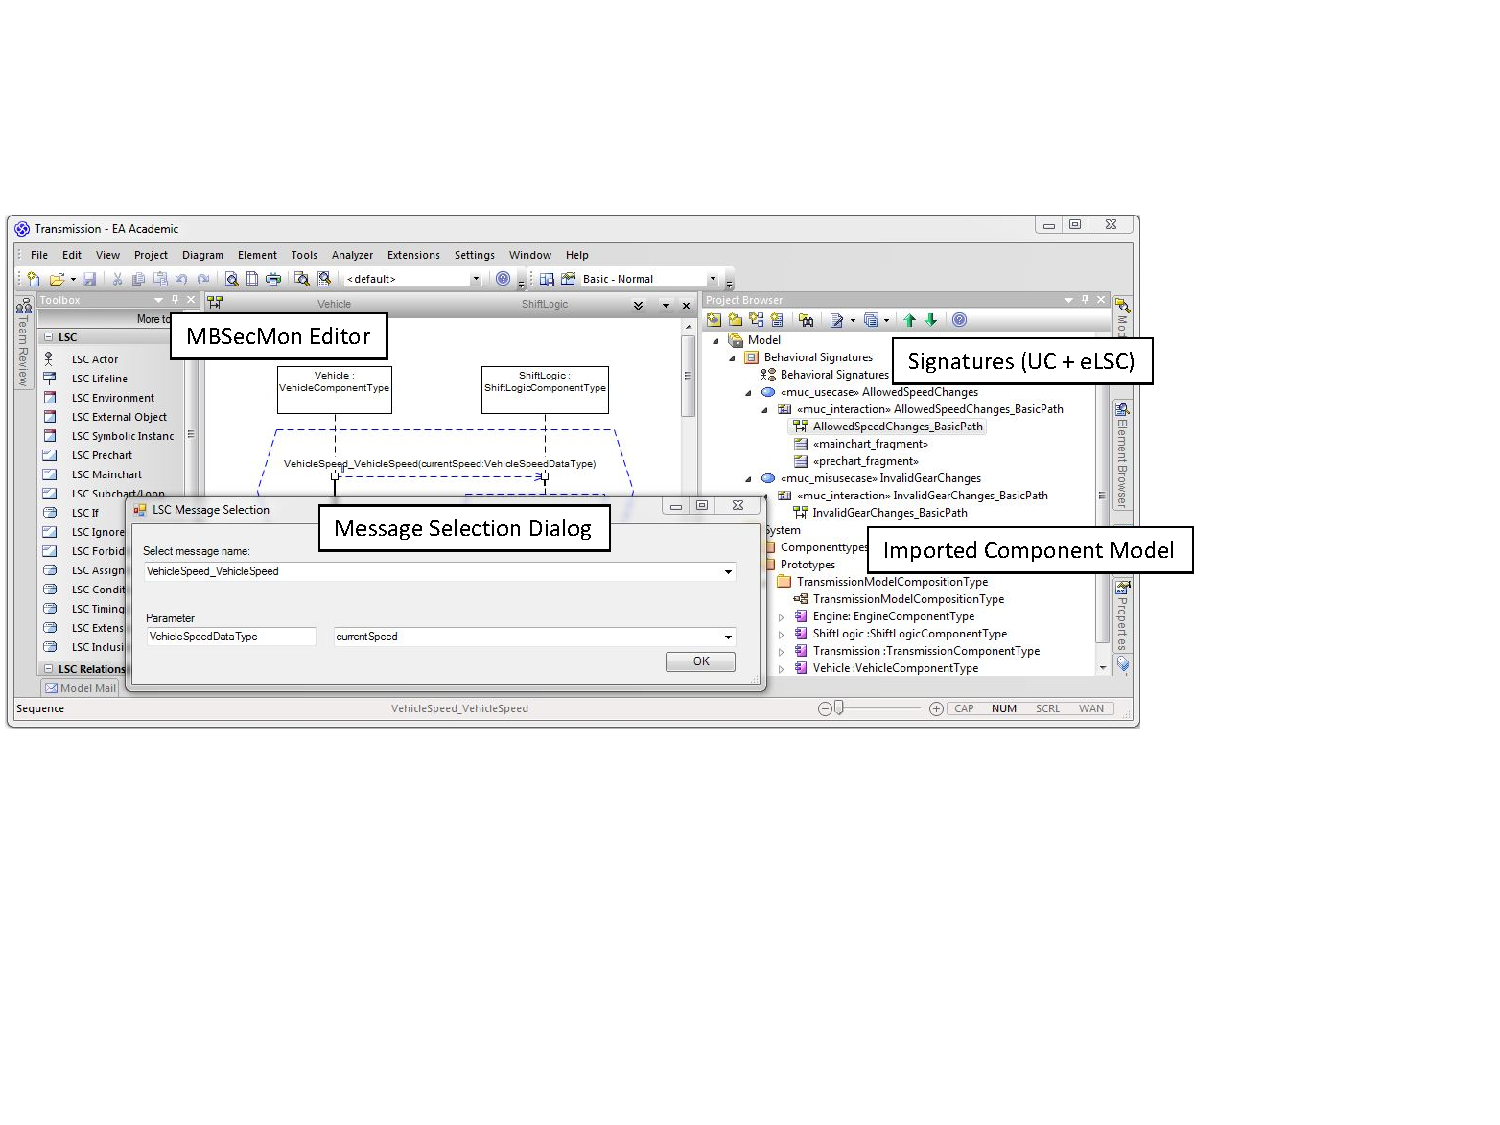
\includegraphics[width=.9\textwidth]{MBSecMonEditor}
  \caption{Tailored Signature Editor for AUTOSAR}
  \label{fig:mbsecmoneditor}
\end{center}
\end{figure}

\textit{MBSecMon process:} 
For this purpose, the MBSecMon specification language (MBSecMonSL), which consists of extended Live Sequence Charts (eLSC) that are structured by use/misuse cases (UC/MUC), is used in the MBSecMon framework.
In addition to the concepts of the wide-spread  Message Sequence Charts~\cite{Harel2004a}, eLSCs distinguish between hot (solid red border) and cold (dashed blue border) elements, where hot elements are mandatory and cold elements are optional.
Furthermore, two forms of eLSCs exist, an universal eLSC with a prechart (precondition) (blue dashed hexagon) before the mainchart (solid black rectangle) and an existential eLSC without a precondition.
In the prechart, every element is interpreted as mandatory.
This is based on the interpretation of the prechart as a precondition.  
When the prechart is fulfilled, the part of the signature in the mainchart is evaluated.

The import of the component view from an AUTOSAR tool to EA forms the basis for the signature modeling.
The MBSecMon EA add-in (Fig.~\ref{fig:mbsecmoneditor}) provides a context sensitive choice of messages between components and their parameter types. 
This ensures the compliance to the modeled AUTOSAR system. 


\begin{figure}[tb]
\begin{center}
  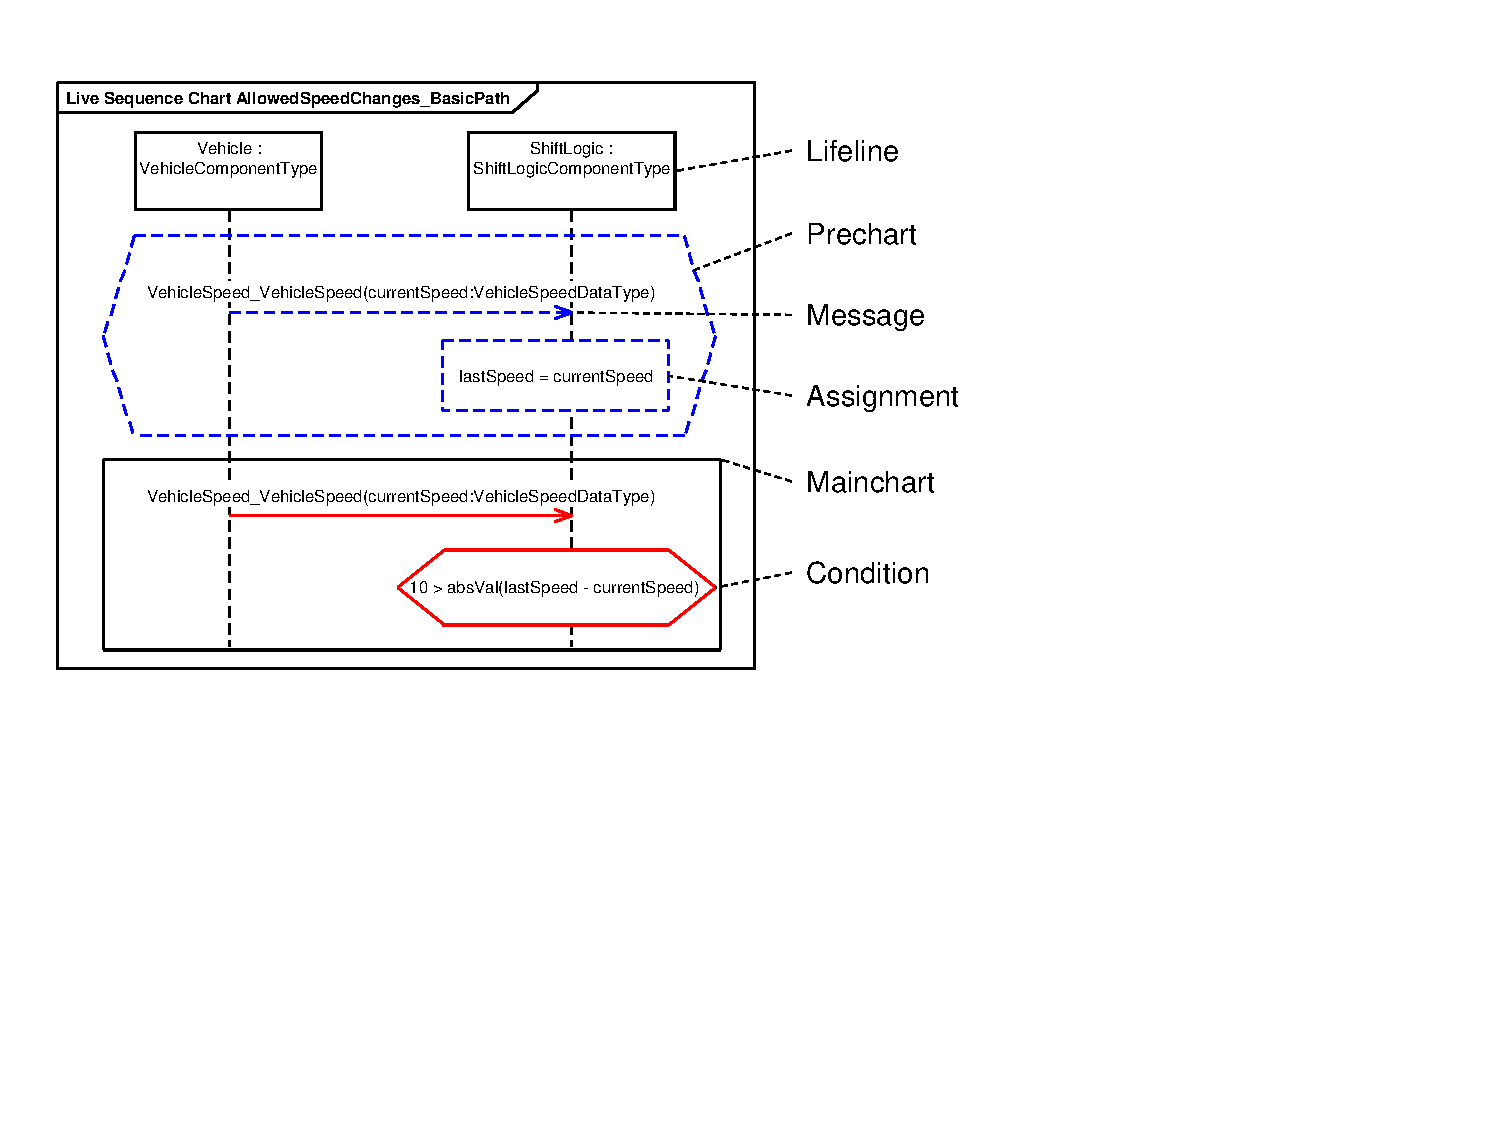
\includegraphics[width=.7\textwidth]{LSCSignatures}
  \caption{Signature of the Use Case ``AllowedSpeedChanges''}
  \label{fig:lscsignatures}
\end{center}
\end{figure}

\textit{Example:} 
Figure~\ref{fig:lscsignatures} shows a simple example of a concurrent signature that uses only the basic elements of the eLSC language.
This signature monitors the communication between the \emph{Vehicle} and the \emph{ShiftLogic} components by initializing the monitor for every message, consisting of a sending and a receiving event, transmitted over the port \emph{VehicleSpeed}.
The message contains the value \emph{currentSpeed} that is stored by the assignment to an eLSC specific variable \emph{lastSpeed}.
The first processed sending event triggers the initialization of a new instance of the signature that concurrently monitors the next messages.
The next \emph{VehicleSpeed} message is processed by the mainchart of the first instance and evaluated by the condition to the previous value stored in \emph{lastSpeed}.
This monitoring instance is then terminated based on the result of the condition. 
Subsequently, the same message is evaluated by the prechart of the second instance of the signature and overwrites the variable \emph{lastSpeed} with the new value. 


\subsubsection{Challenge \ref{itm:mappingsig}: Mapping to platform specific monitoring code.}%$~~$\\
%The signatures modeled in by the MBSecMon EA add-in are exported to a XMI representation based on the MBSecMonSL metamodel~\cite{Patzina2011a} that is used for code generation. 
By modeling signatures on a much more abstract level than the code of the target platform and using an annotation language in the signatures, the code generator needs additional information about the mapping to the target platform. 

\textit{MBSecMon process:} 
To support type safe, AUTOSAR-compliant interfaces for the monitor, additional mappings are generated to the platform specific information (PSI) file. 
It contains mappings between AUTOSAR instrumentation interface and the internal events of the monitor, data types for transferred values, a code mapping of signature annotations to the target domain, and configuration details for the code generation.
Most information for the file can be automatically derived from the imported system specification and the modeled signatures.
Only mappings exported by the EA add-in from annotated pseudo code in the signatures have to be adapted manually to the target language.
For more convenient usage, a mapping library for these annotations could automate this manual step. 

\textit{Example:} 
The generated PSI file provides the mapping of pseudo code used in the signatures to platform-conform code fragments, as depicted in Listing~\ref{lst:lscPSIMapping} for a method \emph{absVal} in the condition of the signature in Fig.~\ref{fig:lscsignatures}.

\lstset{language=XML,
basicstyle=\scriptsize,
mathescape=true,
frame=single,
captionpos=t,
showstringspaces=false}
\begin{lstlisting}[float=tb, caption=LSC specific information in the PSI file, label={lst:lscPSIMapping}]
<entry key="AllowedSpeedChanges_BasicPath.context_method.absVal">fabs
</entry>
\end{lstlisting}

%\textcolor{red}{example for PSI? Example for COHXML?}
%\textcolor{red}{manual changes in PSI file}



\subsubsection{Challenge \ref{itm:connectingmonitors}: Providing communication data to the monitors.}%$~~$\\
The system model of the AUTOSAR specification uses the concept of the Virtual Function Bus (VFB) and only describes the communication pattern (e.g. sender/receiver).
This communication is realized on the target platform depending on the RTE and the allocation of the SW-Cs to the different ECUs.
This hampers the monitoring of the communication between the SW-Cs.

  
\textit{MBSecMon process:}
Based on the signatures, the \emph{instrumenting device} needs a clear naming convention for the monitor interfaces to allow for the wrapping of write and read methods in the AUTOSAR system code. 
Additionally, the \emph{instrumenting device} uses the exported information that specifies, based on the signatures, which ports in the AUTOSAR system have to be instrumented to minimize the footprint of the instrumentation by only adding method calls for the required events.


%The code generation (interfaces and mapping) have been extended to be type save by using the original AUTOSAR data types.
%\textcolor{red}{For code generation, the exported signatures as XMI files are transformed to the intermediate language Monitor Petri nets (MPN).
%This more explicit representation of the signatures are then, together with the platform-specific information, including mappings of events, data types and the replacement of pseudo code, used to generate AUTOSAR conform C code.}

\textit{Example:} 
The interfaces of the monitor are named based on the naming conventions of the AUTOSAR standard.
Thus, the \emph{instrumenting device} can automatically generate calls to the interfaces into the system code.
Listing~\ref{lst:monitorinterfaces} shows the interfaces of the generated example monitor.
The method name is derived by concatenation of the string \texttt{dispatchEvent\_} and the full name of the port of the AUTOSAR component and the data type of the parameter origins from the AUTOSAR model.

\lstset{language=C,
basicstyle=\scriptsize,
mathescape=true,
frame=single,
captionpos=t,
showstringspaces=false}
\begin{lstlisting}[float=tb, caption=Monitor interfaces for the running example, label={lst:monitorinterfaces}]
void dispatchEvent_TransmissionModelCompositionType_Vehicle_
  VehicleSpeed(VehicleSpeedDataType$^*$);
void dispatchEvent_TransmissionModelCompositionType_ShiftLogic_
  VehicleSpeed(VehicleSpeedDataType$^*$);
\end{lstlisting}


%\textcolor{red}{Description of instrumentation concept is missing; with view of paths of two communicating SW-Cs?, instrumentation location, where is the monitor located?}

\subsubsection{Challenge \ref{itm:relocatability}: Supporting the relocatability of software components.} %$~~$\\
One of the important concepts of the AUTOSAR standard is the relocatability of SW-Cs that allows for distributing them to different ECUs without changing the specification.
Due to modeling the monitors on the same abstraction level as the AUTOSAR system specification, the developer of the signatures cannot incorporate information about the final distribution of the SW-Cs.
The code generation process must support the generation of distributed monitors based on the actual distribution of the SW-Cs.
This reduces the run-time overhead for single ECUs and the communication overhead over the buses between the ECUs in contrast to a central monitor.

\textit{MBSecMon process:}
In the MBSecMon generation process, the signatures modeled as eLSCs already contain an affiliation of the events (sending and receiving) to the SW-Cs. 
This affiliation is obtained when the exported signatures are transformed to the intermediate Monitor Petri nets (MPN), and allow for generating distributed monitors based on the SW-C located on the same ECU.
To preserve dependencies between the part monitors (e.g. sending before receiving event of a message), an additional communication between the monitors has to be established.
Therefore, the code generator has been prepared to create identifiers that can be replaced by macro definitions to system communication methods.
          

\textit{Example:} In the example, we use the sender-receiver pattern that directly supports transferability and exchange of AUTOSAR software components.
The two components, \emph{ShiftLogic} and \emph{Vehicle}, in the signature in Fig.~\ref{fig:lscsignatures} can be distributed to different ECUs by defining ``\lstset{basicstyle=\normalsize}\lstinline{ShiftLogic;$\{$Vehicle$\}$}'' in the PSI file the instance that is on the same ECU (\emph{ShiftLogic}) and the instances (\emph{Vehicle}) that is located on another ECU and should be synchronized with it. 

  

\subsubsection{Challenge \ref{itm:minimalOverhead}: Generating monitors with a minimal overhead.} %$~~$\\
The generated run-time monitors are deployed on the ECUs and run alongside the SW-Cs.
Hence, their induced run-time and memory overhead on the ECUs have to be sufficiently small.
The reasonable overhead depends on the required level of safety and security that has to be reached by monitoring.
For the runtime-overhead, a worst case upper bound can be calculated by a static analysis of the signatures in the MPN format.

\textit{Example:} In the presented example in Figure~\ref{fig:lscsignatures} the monitor has to evaluate two transitions per monitor instance (sending or receiving events) in one event processing step.
Additionally, to this computation the annotated assignment or condition has to be taken into account.   

%Hence, they can only add a run-time and memory overhead to the ECUs that is sufficiently small.      
The evaluation in Sect.~\ref{sec:evaluation} shows the overhead that the resulting monitors introduce to the system.





